% LTex: language=pl
\section{Serwer fizyczny}
W ramach przebudowy istniejącego systemu STOS zostały zakupione 2 nowe serwery fizyczne w~ramach przetargu rozpisanego przez Politechnikę Gdańską, na które miał zostać wdrożony system STOS-NEW.

\subsection{Komponenty serwera}
Każdy z tych serwerów zbudowany jest oparty na architekturze AMD64 i~korzysta z chipsetu AMD X670 i~gniazda procesora zgodnego ze specyfikacją AM5 oferowanych przez płytę główną GIGABYTE X670 Gaming v2\cite{gigabyteX670}. Jako procesor wykorzystano kompatybilny z płytą główną procesor AMD Ryzen 9 7950X, posiadający 16 rdzeni i~32 wątki o~bazowym taktowaniu zegara o~częstotliwości $4,5 Ghz$ i~taktowaniem maksymalnym $5,7 Ghz$\cite{ryzen}. Wspiera on maksymalnie $128 GB$ pamięci RAM w~standardzie DDR5, w~tym serwerze zainstalowano zestaw 4 kości, każda o~pojemności $32 GB$, składające się na zestaw Patriot Viper Venom 128GB DDR5, z taktowaniem $6400 Mhz$ i~opóźnieniem CAS wynoszącym 32 cykle zegara (CL32)\cite{patriotRam}. Za chłodzenie procesora odpowiada chłodnica Shadow Rock 3 produkowana przez firmę CoolerMaster, wykorzystująca mechanizm chłodzenia powietrznego\cite{coolermaster}. Na pamięć trwałą serwera składają się 3 dyski, 2 dyski w~technologii M.2 Samsung Evo 990 o~pojemności $1 TB$ każdy\cite{samsungSsd}, i~dysk SSD Silicon Ace A55\cite{sataSsd} o~pojemności $4 TB$, łącznie dające $6 TB$ pamięci trwałej. System zasilany jest zasilaczem Gigabyte UD1000GM PG5, certyfikowanym standardem 80+ Gold i~charakteryzującym się dostarczaną mocą w~wysokości $1 kW$\cite{zasilka}.  Obudową serwera jest obudowa Silver Monkey X Fence SMXC008 z wbudowanym wentylatorem o~średnicy 120 mm\cite{obudowa}.

\subsection{Potencjalne wady konfiguracji sprzętowej}
Pierwszym potencjalnym problemem wynikającym z powyższej specyfikacji sprzętowej jest ograniczenie możliwej do wykorzystania pamięci RAM narzucone przez procesor. W~razie potrzeby zwiększenia dostępnej pamięci operacyjnej na serwerze konieczna jest również wymiana procesora na taką jednostkę, która pozwala na skorzystanie z takiej, większej, ilości pamięci. Kolejnym potencjalnym wąskim gardłem jest zastosowane rozwiązanie chłodzenia procesora. Chłodnica wykorzystana w~serwerze, CoolerMaster Shadow Rock 3, według specyfikacji, jest w~stanie skutecznie utrzymać akceptowalną temperaturę procesora o~mocy do $190 W$, wyrażanej jako TDP (Thermal Design Power), oznaczająca maksymalne zużycie mocy przez komponent, w~tym przypadku procesor, które należy brać pod uwagę przy projektowaniu systemu\cite{intelTdp}. AMD Ryzen 7950X, przy bazowym taktowaniu zegara, szacowany jest przez producenta na charakteryzujący się mocą $170 W$ TDP. Sam zapas $20W$ jest wystarczający w~przypadku chłodzenia procesora, lecz w~przypadku Ryzena 7950X pracującego w~trybie boost, jego zużycie energii jest w~stanie dochodzić do ok. $230 W$ - $250 W$\cite{amdPpt, testyMocy}, co jest równoznaczne z deficytem mocy chłodnicy rzędu od $40W$ do $60W$. Zastosowanie obecnego chłodzenia może, z dużym prawdopodobieństwem, doprowadzić do powstania efektu znanego jako „thermal throttling”\cite{throttling}. Polega on na ograniczaniu mocy i~prędkości procesora, gdy osiąga on temperatury dochodzące do maksymalnych dopuszczalnych przez producenta temperatur, mieszczących się zazwyczaj w~zakresie od $95^{\circ}\mathrm{C}$ do $105^{\circ}\mathrm{C}$. W~przypadku powyższej konfiguracji, efekt ten powstawać będzie przy zwiększonym obciążeniu serwera, uniemożliwiając procesorowi wykorzystanie w~pełni jego potencjału taktowania. Dodatkowym czynnikiem jest stosunkowo niska objętość powietrza odprowadzanego ze środka obudowy serwera, za którą odpowiedzialny jest jeden wiatrak o~średnicy 120 mm. Warto nadmienić, że są to jedynie rozważania teorytyczne i~w~celu ustalenia faktycznej wydajności zastosowanego chłodzenia, należałoby przeprowadzić odpowiednie testy serwera, które nie znajdują się w~zakresie tego projektu.

\begin{figure}[!h]
	\begin{center}
		\resizebox{0.7\textwidth}{!} {
			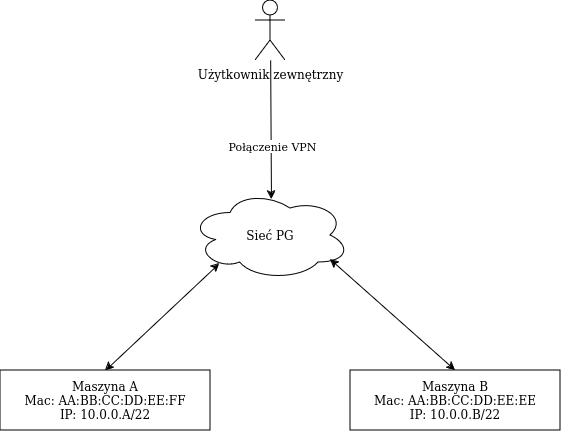
\includegraphics{img/4/fizycznaSiec.png}
		}
		\caption[Diagram fizycznego rozmieszczenia maszyn w~sieci Politechniki Gdańskiej]{Diagram przedstawiający umiejscowienie maszyn fizycznych w~sieci Politechniki Gdańskiej. Adresy IP i~adresy MAC nie są faktycznymi adresami maszyn w~sieci. Źródło własne.}
		\label{diagramSiecFizyczna}
	\end{center}
\end{figure}

\subsection{Serwery w~kontekście sieci Politechniki Gdańskiej}
Obie maszyny fizyczne znajdują się na terenie Politechniki Gdańskiej i~znajdują się w~sieci wewnętrznej PG. Posiadają one statycznie przypisane z poziomu sieci adresy IP, odpowiadające adresom MAC ich kart sieciowych. Dostęp z sieci zewnętrznych odbywa się za pomocą VPN Politechniki Gdańskiej i~uzyskaniu dostępu do sieci politechnicznej. Topologię maszyn fizycznych w~kontekście sieci przedstawia diagram \ref{diagramSiecFizyczna}.

